\documentclass[size=a4, parskip=half, titlepage=false, toc=flat, toc=bib, 12pt]{scrartcl}

\setuptoc{toc}{leveldown}

% Ajuste de las líneas y párrafos
\linespread{1.2}
\setlength{\parindent}{0pt}
\setlength{\parskip}{12pt}

% Español
\usepackage[spanish, es-tabla]{babel}

% Matemáticas
\usepackage{amsmath}
\usepackage{amsthm}

% Links
%\usepackage{hyperref}

% Fuentes
\usepackage{newpxtext,newpxmath}
\usepackage[scale=.9]{FiraMono}
\usepackage{FiraSans}
\usepackage[T1]{fontenc}

\defaultfontfeatures{Ligatures=TeX,Numbers=Lining}
\usepackage[activate={true,nocompatibility},final,tracking=true,factor=1100,stretch=10,shrink=10]{microtype}
\SetTracking{encoding={*}, shape=sc}{0}

\usepackage{graphicx}
\usepackage{float}

% Mejores tablas
\usepackage{booktabs}

\usepackage{adjustbox}

% COLORES

\usepackage{xcolor}

\definecolor{verde}{HTML}{007D51}
\definecolor{esmeralda}{HTML}{045D56}
\definecolor{salmon}{HTML}{FF6859}
\definecolor{amarillo}{HTML}{FFAC12}
\definecolor{morado}{HTML}{A932FF}
\definecolor{azul}{HTML}{0082FB}
\definecolor{error}{HTML}{b00020}

% ENTORNOS
\usepackage[skins, listings, theorems]{tcolorbox}

\newtcolorbox{recuerda}{
  enhanced,
%  sharp corners,
  frame hidden,
  colback=black!10,
	lefttitle=0pt,
  coltitle=black,
  fonttitle=\bfseries\sffamily\scshape,
  titlerule=0.8mm,
  titlerule style=black,
  title=\raisebox{-0.6ex}{\small RECUERDA}
}

\newtcolorbox{nota}{
  enhanced,
%  sharp corners,
  frame hidden,
  colback=black!10,
	lefttitle=0pt,
  coltitle=black,
  fonttitle=\bfseries\sffamily\scshape,
  titlerule=0.8mm,
  titlerule style=black,
  title=\raisebox{-0.6ex}{\small NOTA}
}

\newtcolorbox{error}{
  enhanced,
%  sharp corners,
  frame hidden,
  colback=error!10,
	lefttitle=0pt,
  coltitle=error,
  fonttitle=\bfseries\sffamily\scshape,
  titlerule=0.8mm,
  titlerule style=error,
  title=\raisebox{-0.6ex}{\small ERROR}
}

\newtcblisting{shell}{
  enhanced,
  colback=black!10,
  colupper=black,
  frame hidden,
  opacityback=0,
  coltitle=black,
  fonttitle=\bfseries\sffamily\scshape,
  %titlerule=0.8mm,
  %titlerule style=black,
  %title=Consola,
  listing only,
  listing options={
    style=tcblatex,
    language=sh,
    breaklines=true,
    postbreak=\mbox{\textcolor{black}{$\hookrightarrow$}\space},
    emph={jmml@UbuntuServer, jmml@CentOS},
    emphstyle={\bfseries},
  },
}

\newtcbtheorem[number within=section]{teor}{\small TEOREMA}{
  enhanced,
  sharp corners,
  frame hidden,
  colback=white,
  coltitle=black,
  fonttitle=\bfseries\sffamily,
  %separator sign=\raisebox{-0.65ex}{\Large\MI\symbol{58828}},
  description font=\itshape
}{teor}

\newtcbtheorem[number within=section]{prop}{\small PROPOSICIÓN}{
  enhanced,
  sharp corners,
  frame hidden,
  colback=white,
  coltitle=black,
  fonttitle=\bfseries\sffamily,
  %separator sign=\raisebox{-0.65ex}{\Large\MI\symbol{58828}},
  description font=\itshape
}{prop}

\newtcbtheorem[number within=section]{cor}{\small COROLARIO}{
  enhanced,
  sharp corners,
  frame hidden,
  colback=white,
  coltitle=black,
  fonttitle=\bfseries\sffamily,
  %separator sign=\raisebox{-0.65ex}{\Large\MI\symbol{58828}},
  description font=\itshape
}{cor}

\newtcbtheorem[number within=section]{defi}{\small DEFINICIÓN}{
  enhanced,
  sharp corners,
  frame hidden,
  colback=white,
  coltitle=black,
  fonttitle=\bfseries\sffamily,
  %separator sign=\raisebox{-0.65ex}{\Large\MI\symbol{58828}},
  description font=\itshape
}{defi}

\newtcbtheorem{ejer}{\small EJERCICIO}{
  enhanced,
  sharp corners,
  frame hidden,
  left=0mm,
  right=0mm,
  colback=white,
  coltitle=black,
  fonttitle=\bfseries\sffamily,
  %separator sign=\raisebox{-0.65ex}{\Large\MI\symbol{58828}},
  description font=\itshape,
  nameref/.style={},
}{ejer}

% CÓDIGO
\usepackage{listings}

% CABECERAS
\pagestyle{headings}
\setkomafont{pageheadfoot}{\normalfont\normalcolor\sffamily\small}
\setkomafont{pagenumber}{\normalfont\sffamily}

% ALGORITMOS
\usepackage[vlined,linesnumbered]{algorithm2e}
\usepackage{listings}
\usepackage{color}
\renewcommand{\lstlistingname}{Listado}

\definecolor{dkgreen}{rgb}{0,0.6,0}
\definecolor{gray}{rgb}{0.5,0.5,0.5}
\definecolor{mauve}{rgb}{0.58,0,0.82}

\lstset{frame=tb,
  language=Python,
  aboveskip=3mm,
  belowskip=3mm,
  showstringspaces=false,
  columns=flexible,
  basicstyle={\small\ttfamily},
  numbers=none,
  numberstyle=\tiny\color{gray},
  keywordstyle=\color{blue},
  commentstyle=\color{dkgreen},
  stringstyle=\color{mauve},
  breaklines=true,
  breakatwhitespace=true,
  tabsize=2
}

% Formato de los pies de figura
\setkomafont{captionlabel}{\scshape}
\SetAlCapFnt{\normalfont\scshape}
\SetAlgorithmName{Algoritmo}{Algoritmo}{Lista de algoritmos}

% BIBLIOGRAFÍA
%\usepackage[sorting=none]{biblatex}
%\addbibresource{bibliografia.bib}

\begin{document}

\renewcommand{\proofname}{\normalfont\sffamily\bfseries\small DEMOSTRACIÓN}

\title{Trabajo 1\\
Programación}
\subject{Aprendizaje automático}
\author{Johanna Capote Robayna\\
    5 del Doble Grado en Informática y Matemáticas\\
    Grupo A}
\date{}
\publishers{\vspace{2cm}
\includegraphics[height=2.5cm]{UGR}\vspace{1cm}}
\maketitle

\newpage

\tableofcontents
\newpage

\section{Gradiente descendente}
Este ejercicio se desarrolla en el archivo \verb|p1_ej1.py|.
\begin{enumerate}
\item Implementar el algoritmo de gradiente descendente.

Para implementar el algoritmo definimos la función \verb|gd| a la cuyos argumentos son:
\begin{itemize}
\item \textbf{w}: punto inicial del algoritmo
\item \textbf{lr}: tasa de aprendizaje.
\item \textbf{grad\_fun}: gradiente de la función.
\item \textbf{fun}: función sobre la que itera el algoritmo.
\item \textbf{epsilon}: umbral de parada del algoritmo.
\item \textbf{max\_iters}: número de máximo de iteraciones que realiza el algoritmo en caso
de que no se satisfaga los criterios de parada.
\end{itemize}

\begin{lstlisting}
def gd(w, lr, grad_fun, fun, epsilon, max_iters = MAX_ITER):
	for it in range(max_iters):
		if(fun(w) < epsilon):
			break
		w = w - lr * grad_fun(w)

	return w, it
\end{lstlisting}
\item Considerar la función $E(u,v) = (ue^v - 2ve^{-u})^2$. Usar gradiente descendente
para encontrar un mínimo de esta función, comenzando desde el punto $(u,v) = (1,1)$ y usando
una tasa de aprendizaje $\eta = 0.1$.
\begin{enumerate}
\item Calcular analíticamente y mostrar la expresión del gradiente de la función $E(u, v)$.

Calculamos las derivadas parciales de la función $E(u,v) = (ue^v - 2ve^{-u})^2$:
$$ \frac{\partial}{\partial u} E(u,v) = 2 e^{-2 u} (e^{u + v} u - 2 v) (e^{u + v} + 2 v) $$
$$ \frac{\partial}{\partial v} E(u,v) = 2 e^{-2 u} (-2 + e^{u + v} u) (e^{u + v} u - 2 v)$$

\item ?`Cuántas iteraciones tarda el algoritmo en obtener por primera vez un valor de E(u, v)
inferior a $10^{−14}$?

Ejecutamos el algoritmo de gradiente descendente con punto inicial $(1,1)$, tasa de aprendizaje $\eta = 0.1$
y $\epsilon = 10^{-14}$. Tras la ejecución vemos que tarda \textbf{10 iteraciones} en obtener un valor inferior
a $10^{-14}$.

\item ?`En qué coordenadas (u, v) se alcanzó por primera vez un valor igual o menor a $10^{−14}$
en el apartado anterior ?

\spanishdecimal{.}
En las coordenadas $( 0.0447 ,  0.0239 )$ se alcanzó por primera vez un valor
menor o igual a $10^{-14}$.
\end{enumerate}

\item Considerar ahora la función $f(x,y) = (x-2)^2 + 2(y + 2)^2 + 2 \sin(2 \pi x) \sin(2 \pi y)$

En primer lugar calculamos las derivadas parciales de la funcion $f(x,y)$
$$\frac{\partial}{\partial x} f(x,y) =  2 (x - 2 + 2 \pi \cos(2 \pi x) \sin(2 \pi y))$$
$$\frac{\partial}{\partial y} f(x,y) = 4 (2 + y + \pi \cos(2 \pi y) \sin(2 \pi x))$$
\begin{enumerate}
\spanishdecimal{.}
\item Usar gradiente descendente para minimizar esta función. Usar como punto inicial
$(x_0 = 1, y_0 = −1)$, (tasa de aprendizaje $\eta = 0.01$ y un máximo de 50 iteraciones.
Generar un gráfico de cómo desciende el valor de la función con las iteraciones. Repetir
el experimento pero usando $\eta = 0.1$, comentar las diferencias y su dependencia de $\eta$.

Ejecutamos en primer lugar el algoritmode gradiente descendente con punto inicial $(1, -1)$, tasa
de aprendizaje $\eta = 0.01$ y un máximo de 50 iteraciones, obteniendo la siguiente gráfica:

\begin{figure}[H]
\centering
\spanishdecimal{.}
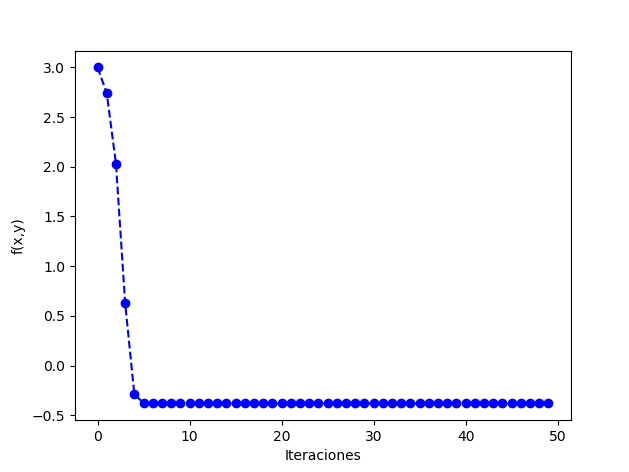
\includegraphics[width=0.7\textwidth]{./img/lr001}
\caption{Tasa de aprendizaje $\eta = 0.01$.}
\end{figure}
A continuación repetimos el experimento cambiando el parámetro de tasa de aprendizaje por $\eta = 0.1$,
obteniendo:

\begin{figure}[H]
\centering
\spanishdecimal{.}
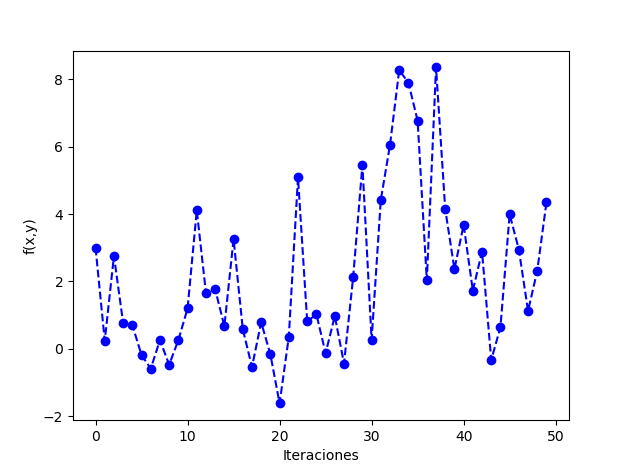
\includegraphics[width=0.7\textwidth]{./img/lr01}
\caption{Tasa de aprendizaje $\eta = 0.1$.}
\end{figure}
\spanishdecimal{.}
Si comparamos las dos gráficas vemos que con una tasa de aprendizaje $\eta = 0.01$ la función
converge rápidamente en menos de 10 iteraciones, mientras que una tasa de aprendizaje $\eta = 0.1$ ya es un
valor muy grande y hace que la función oscile sin llegar a converger. Observamos también que con
una tasa de aprendizaje mayor consigue valores más pequeños que el mínimo alcanzado con $\eta = 0.01$,
pero sin embargo no se estabiliza.

Es por esto que en este caso una tasa de aprendizaje de $\eta = 0.1$ es
demasiado elevada y depende del número de iteraciones que acabe en un punto mayor o menor, mientras que
con una tasa de $\eta = 0.01$ el algoritmo converge rápido y alcanza un mínimo aunque dependa del
punto inicial para que sea el mínimo absoluto.

\begin{figure}[H]
\centering
\spanishdecimal{.}
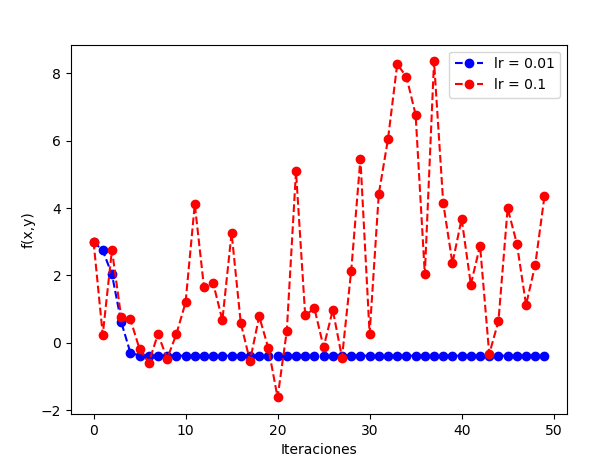
\includegraphics[width=0.7\textwidth]{./img/lr}
\caption{Comparación de las dos gráficas $\eta = 0.01$ y $\eta = 0.1$.}
\end{figure}
\spanishdecimal{.}
\item Obtener el valor mínimo y los valores de las variables (x, y) en donde se alcanzan
cuando el punto de inicio se fija en: $(2.1, −2.1)$, $(3, −3)$, $(1.5, 1.5)$, $(1, −1)$. Generar una
tabla con los valores obtenidos.

Se ha ejecutado el algoritmo con una tasa de aprendizaje $\eta = 0.01$.
\begin{table}[H]
\centering
\spanishdecimal{.}
\begin{tabular}{@{}ccc@{}}
\toprule
Punto inicio   & valor mínimo                    & ( x, y )                                 \\ \midrule
$(2.1 , -2.1)$ & {\color[HTML]{000000} $-1.820$} & {\color[HTML]{000000} $(2.244, -2.238)$} \\ \midrule
$(3, -3)$      & {\color[HTML]{000000} $-0.3812$} & {\color[HTML]{000000} $(2.731, -2.713)$} \\ \midrule
$(1.5, 1.5)$   & {\color[HTML]{000000} $18.042$} & {\color[HTML]{000000} $(1.779, 1.031)$}  \\ \midrule
$(1, -1)$      & {\color[HTML]{000000} $-0.381$} & {\color[HTML]{000000} $(1.269, -1.287)$} \\ \bottomrule
\end{tabular}
\end{table}
Podemos observar que el valor mínimo que alcanza el algoritmo depende fuertemente del punto inicial, esto
es debido a la naturaleza de la función que, como veremos en la siguiente imagen, tiene muchos mínimos locales y
como nuestra tasa de aprendizaje es pequeña converge rápidamente al mínimo local más cercano.
\begin{figure}[H]
\centering
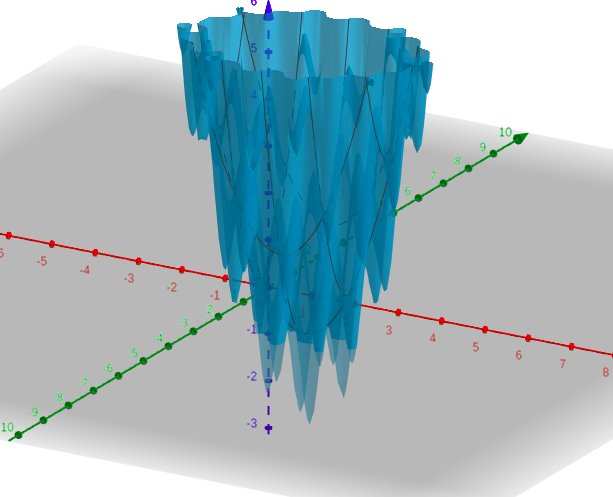
\includegraphics[width=0.7\textwidth]{./img/fxy}
\caption{Función $f(x,y)$ dibujada con Geogebra.}
\end{figure}
\end{enumerate}
\item ?`Cuál sería su conclusión sobre la verdadera dificultad de encontrar el mínimo
global de una función arbitraria?

La verdadera dificultad a la hora de encontrar el mínimo global en una función arbitraria
es ajustar los parámetros del algoritmo: la tasa de aprendizaje y el punto inicial.

Por una parte si escogemos una \textbf{tasa de aprendizaje} muy elevada puede ser que el algoritmo converja
muy despacio o que oscile y nunca alcance un mínimo, mientras que una tasa demasiado pequeña puede hacer
que el algoritmo converja demasiado rápido cayendo en mínimos locales. Esta claro que es difícil dar con
el valor exacto de la tasa de aprendizaje para que el algoritmo converja correctamente al mínimo absoluto,
una solución a este problema podría ser un valor iterativo de tasa de aprendizaje, comenzando con un valor
muy elevado para poder ``explorar'' al principio la función y disminuyendo el valor de la tasa de aprendizaje
iterativamente para ayudar al algoritmo a converger hacía un mínimo.

Por otra parte elegir un \textbf{punto inicial} adecuado puede ser clave, ya que como vimos en nuestro experimento
si elegiamos un punto muy alejado del mínimo absoluto, al estar este rodeado de mínimos locales el algoritmo
converge a uno de estos.
\end{enumerate}

\section{Regresión lineal}
Este ejercicio se ha desarrollado en el archivo \verb|p1_ej2.py|.
\begin{enumerate}

\item Estimar un modelo de regresión lineal a partir de los datos proporcionados de
dichos números usando tanto el algoritmo de la pseudo-inversa como Gradiente descendente
estocástico (SGD). Las etiquetas serán $\{−1, 1\}$, una para cada vector de cada uno de los
números. Pintar las soluciones obtenidas junto con los datos usados en el ajuste. Valorar
la bondad del resultado usando $E_{in}$ y $E_{out}$.

\spanishdecimal{.}
Ejecutamos el algoritmo de gradiente descendente estocástico y pintamos los resultados.
En primer lugar ejecutamos el algoritmo de gradiente descendente estocástico con parámetros:
\begin{itemize}
\item \textbf{x}: vector de características que nos proporciona el ejercicio.
\item \textbf{y}: vector de etiquetas que nos proporciona el ejercicio.
\item \textbf{lr}: tasa de aprendizaje $\eta = 0.01$
\item \textbf{max\_iters}: número máximo de iteraciones $20000$.
\item \textbf{tam\_minibatch}: tamaño 32.
\item \textbf{\footnote{Parámetro añadido. Este parámetro indica el tamaño del vector w,
el cual cambia su tamaño en el último experimento.}{tam}}: por defecto esta a 3, cambiará
su valor en el último experimento.

Obtenemos como resultados:
\begin{lstlisting}
Bondad del resultado para grad. descendente estocastico:

Ein:  0.07996130732163849
Eout:  0.13396594439564616
\end{lstlisting}
\end{itemize}
\begin{figure}[H]
\centering
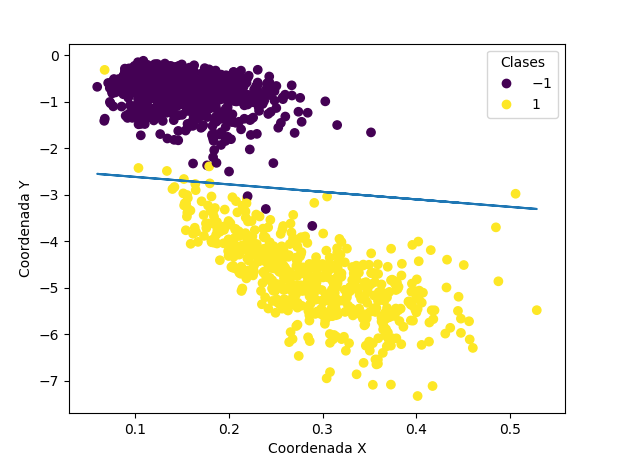
\includegraphics[width=0.7\textwidth]{./img/ej21}
\caption{Algoritmo de gradiente descendente estocástico.}
\end{figure}

Ejecutamos a continuación el algoritmo de la pseudo-inversa con los datos proporcionado para
el ejercicio y obtenemos:
\begin{lstlisting}
Bondad del resultado para el algoritmo de la pseudoinversa:

Ein:  0.07918658628900395
Eout:  0.13095383720052586
\end{lstlisting}

\begin{figure}[H]
\centering
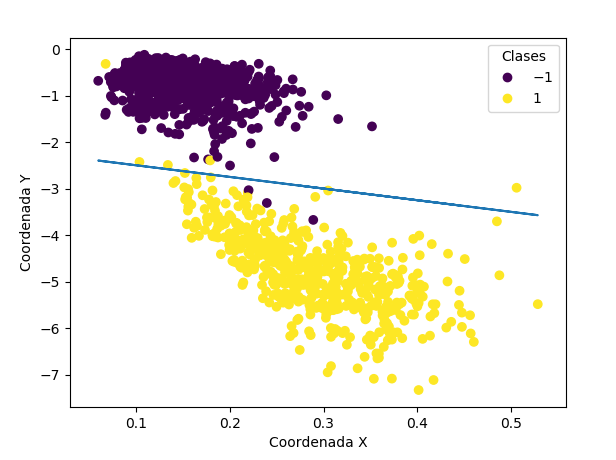
\includegraphics[width=0.7\textwidth]{./img/ej22}
\caption{Algoritmo de la pseudo-inversa.}
\end{figure}

\begin{figure}[H]
\centering
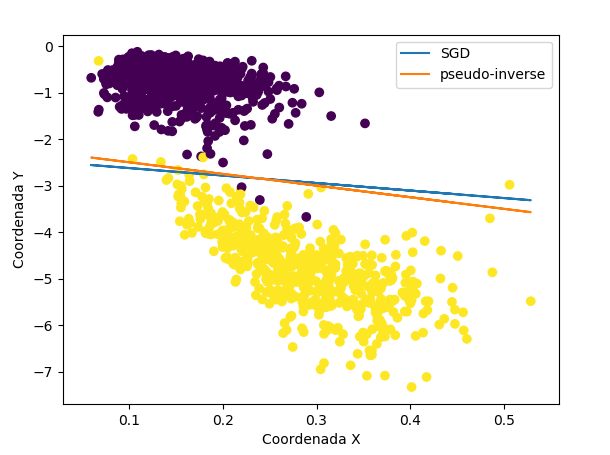
\includegraphics[width=0.7\textwidth]{./img/ej222}
\caption{Comparación entre gradiente descendente estocastico y pseudo-inversa.}
\end{figure}

\item En este apartado exploramos como se transforman los errores $E_{in}$ y $E_{out}$ cuando
aumentamos la complejidad del modelo lineal usado.

\begin{enumerate}

\item Generar una muestra de entrenamiento de $N = 1000$ puntos en el cuadrado
$X = [−1, 1] × [−1, 1]$. Pintar el mapa de puntos 2D.

Para ello se ha definido la función \verb|simula_unif|. La ejecutamos y pintamos el resultado.

\begin{figure}[H]
\centering
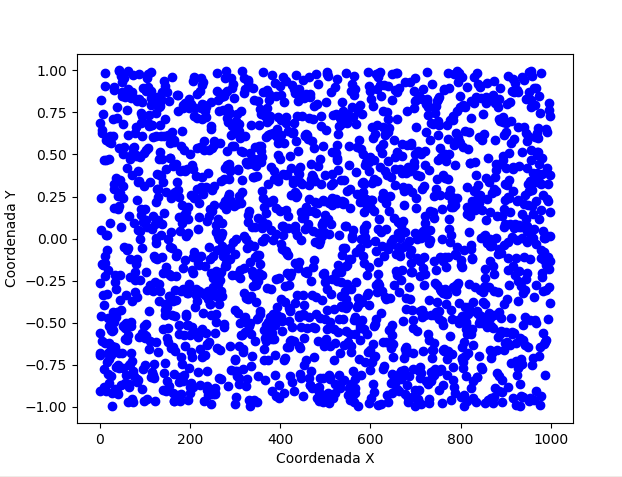
\includegraphics[width=0.7\textwidth]{./img/ej23}
\caption{Muestra de $1000$ puntos distribuidos en el cuadrado $X = [-1,1]x[-1,1]$.}
\end{figure}

\spanishdecimal{.}
\item Consideremos la función $f (x_1 , x_2 ) = sign((x_1 − 0.2)^2 + x_2^2 − 0.6)$ que usaremos
para asignar una etiqueta a cada punto de la muestra anterior. Introducimos
ruido sobre las etiquetas cambiando aleatoriamente el signo de un $10 \%$ de las
mismas. Pintar el mapa de etiquetas obtenido.

Para este apartado se ha definido la función \verb|genera_conjunto| , que además de fabricar
las etiquetas con la función que nos han proporcionado y añadiendo un ruido del $10 \%$, también
aprovechamos para añadir un $1$ al principio del vector de características $x$. Lo ejecutamos
y los resultados obtenidos son:

\begin{figure}[H]
\centering
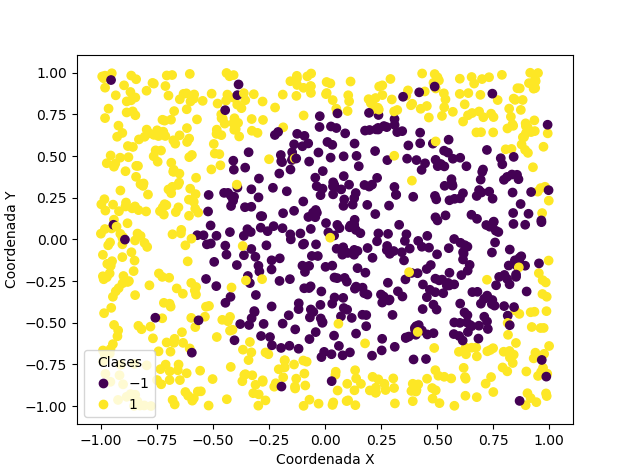
\includegraphics[width=0.7\textwidth]{./img/ej24}
\caption{Muestra etiquetada.}
\end{figure}

\item Usando como vector de características $(1, x_1 , x_2 )$ ajustar un modelo de regresión
lineal al conjunto de datos generado y estimar los pesos $w$. Estimar el error de
ajuste $E_{in}$ usando Gradiente Descendente Estocástico (SGD).

Como en el apartado anterior ya le añadimos el $1$ al vector de características ejecutamos
el algoritmo de gradiente descendente estocástico con estos datos y con: $\eta = 0.01$, iteraciones
máximas $20000$ y tamaño del \textit{minibatch} 32. Obtenemos los siguientes resultados:

\begin{lstlisting}
Muestra N = 1000, cuadrado [-1,1]x[-1,1]
Bondad del resultado para grad. descendente estocastico:

Ein:  0.9017328368880705
\end{lstlisting}
\begin{figure}[H]
\centering
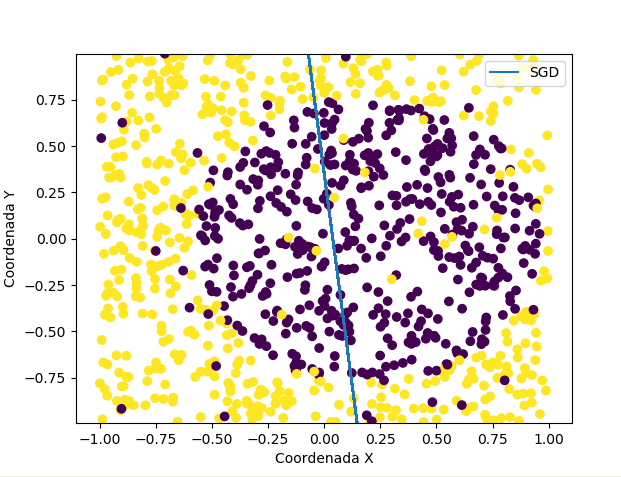
\includegraphics[width=0.7\textwidth]{./img/ej25}
\caption{Algoritmo de gradiente descendente estocástico.}
\end{figure}

\item Ejecutar todo el experimento definido por (a)-(c) 1000 veces (generamos 1000
muestras diferentes) y calcular el valor medio de los errores $E_{in}$ de las 1000 muestras.

Repetimos el experimento anterior en un bucle de $1000$ iteraciones fabricando de nuevo en cada
iteración los conjuntos de datos y al finalizar calculamos los errores medios, obteniendo:

\begin{lstlisting}
Errores Ein y Eout medios tras 1000reps del experimento:

Ein media:  0.909014264842863
Eout media:  0.9149857744864048
\end{lstlisting}

\item Valore que tan bueno considera que es el ajuste con este modelo lineal a la vista
de los valores medios obtenidos de $E_{in}$ y $E_{out}$.
\end{enumerate}
\begin{itemize}
\item Repetir el mismo experimento anterior pero usando características no lineales. Ahora
usaremos el siguiente vector de características: $\Phi_2 (x) = (1, x_1 , x_2 , x_1 x_2 , x^2_1 , x_2^2 )$. Ajustar
el nuevo modelo de regresión lineal y calcular el nuevo vector de pesos ŵ. Calcular
los errores promedio de $E_{in}$ y $E _{out}$.

Para este apartado se ha definido una función \verb|aniade_caract| cuya función es añadir
las características al vector x. Ejecutando de nuevo el experimento con este cambio obtenemos
los siguientes resultados:

\begin{lstlisting}
Errores Ein y Eout medios tras 1000reps del experimento con más características:

Ein media:  0.5704825441885348
Eout media:  0.5759666841725378
\end{lstlisting}

\item A la vista de los resultados de los errores promedios $E_{in}$ y $E_{out}$ obtenidos en los dos
experimentos ?`Que modelo considera que es el más adecuado? Justifique la decisión.

\end{itemize}
\end{enumerate}

\section{BONUS}

\textbf{Método de Newton}. Implementar el algoritmo de minimización de Newton
y aplicarlo a la función $f (x, y)$ dada en el ejercicio.3. Desarrolle los mismos experimentos
usando los mismos puntos de inicio.

Este ejercicio se ha desarrollado en el archivo \verb|bonus.py|.

\begin{figure}[H]
\centering
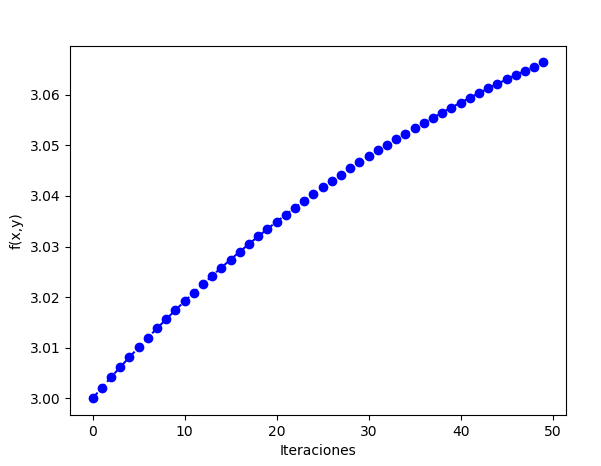
\includegraphics[width=0.7\textwidth]{./img/bonus21}
\caption{Tasa de aprendizaje $\eta = 0.01$}
\end{figure}

\begin{figure}[H]
\centering
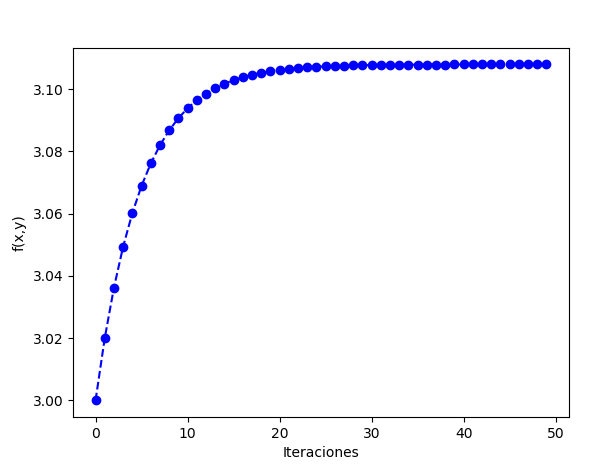
\includegraphics[width=0.7\textwidth]{./img/bonus22}
\caption{Tasa de aprendizaje $\eta = 0.1$}
\end{figure}

\begin{figure}[H]
\centering
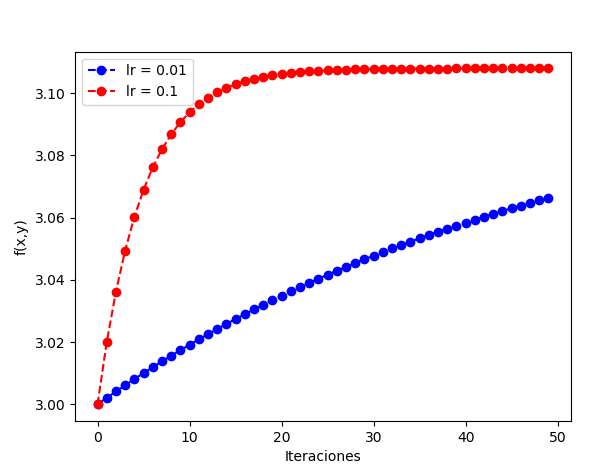
\includegraphics[width=0.7\textwidth]{./img/bonus23}
\caption{Comparación entre las dos tasas de aprendizaje.}
\end{figure}

\begin{table}[H]
\spanishdecimal{.}
\centering
\begin{tabular}{ccc}
\hline
Punto inicio   & valor del óptimo obtenido                    & ( x, y )                                 \\ \hline
$(2.1 , -2.1)$ & {\color[HTML]{000000} $-0.058$} & {\color[HTML]{000000} $(2.028, -2.028)$} \\ \hline
$(3, -3)$      & {\color[HTML]{000000} $3.093$}  & {\color[HTML]{000000} $(3.033, -3.017)$} \\ \hline
$(1.5, 1.5)$   & {\color[HTML]{000000} $24.974$} & {\color[HTML]{000000} $(1.373, 1.516)$}  \\ \hline
$(1, -1)$      & {\color[HTML]{000000} $3.093$}  & {\color[HTML]{000000} $(0.967, -0.983)$} \\ \hline
\end{tabular}
\end{table}

%printbibliography

\end{document}
